% ****** Start of file langevin.tex ******
%%
\documentclass[%
 reprint,
%superscriptaddress,
%groupedaddress,
%unsortedaddress,
%runinaddress,
%frontmatterverbose, 
%preprint,
%showpacs,preprintnumbers,
%nofootinbib,
%nobibnotes,
%bibnotes,
 amsmath,amssymb,
 aps,
%pra,
%prb,
%rmp,
%prstab,
%prstper,
%floatfix,
]{revtex4-1}

\usepackage{graphicx}% Include figure files
\usepackage{dcolumn}% Align table columns on decimal point
\usepackage{bm}% bold math
\usepackage{subcaption}
\usepackage{float}
%\usepackage{hyperref}% add hypertext capabilities
%\usepackage[mathlines]{lineno}% Enable numbering of text and display math
%\linenumbers\relax % Commence numbering lines

%\usepackage[showframe,%Uncomment any one of the following lines to test 
%%scale=0.7, marginratio={1:1, 2:3}, ignoreall,% default settings
%%text={7in,10in},centering,
%%margin=1.5in,
%%total={6.5in,8.75in}, top=1.2in, left=0.9in, includefoot,
%%height=10in,a5paper,hmargin={3cm,0.8in},
%]{geometry}
\DeclareMathOperator\erf{erf}
\DeclareMathOperator\erfc{erfc}
\begin{document}

\preprint{APS/123-QED}

\title{Intensity Distribution of a Dilute Solution of Point Emitters under Gaussian Detection}

\author{Helmut H. Strey}
 \affiliation{Biomedical Engineering Department and Laufer Center for Physical and Quantitative Biology, Stony Brook University, Stony Brook NY 11794-5281.}%Lines break automatically or can be forced with \\

\date{\today}% It is always \today, today,
             %  but any date may be explicitly specified

\begin{abstract}
\begin{description}
\item[PACS numbers]
May be entered using the \verb+\pacs{#1}+ command.
\end{description}
\end{abstract}

\pacs{Valid PACS appear here}% PACS, the Physics and Astronomy
                             % Classification Scheme.
%\keywords{Suggested keywords}%Use showkeys class option if keyword
                              %display desired
\maketitle

%\tableofcontents
\onecolumngrid
\subsection{Introduction}
One strategy to accurately measure the concentration of a dilute solution of fluorecent molecules is to employ the properties of the Poisson distribution.  The basic idea of this method is illustrated in Fig. \cite{poissonconc}.  
\begin{figure}[H]
\begin{center}
\resizebox{.9\textwidth}{!}{%
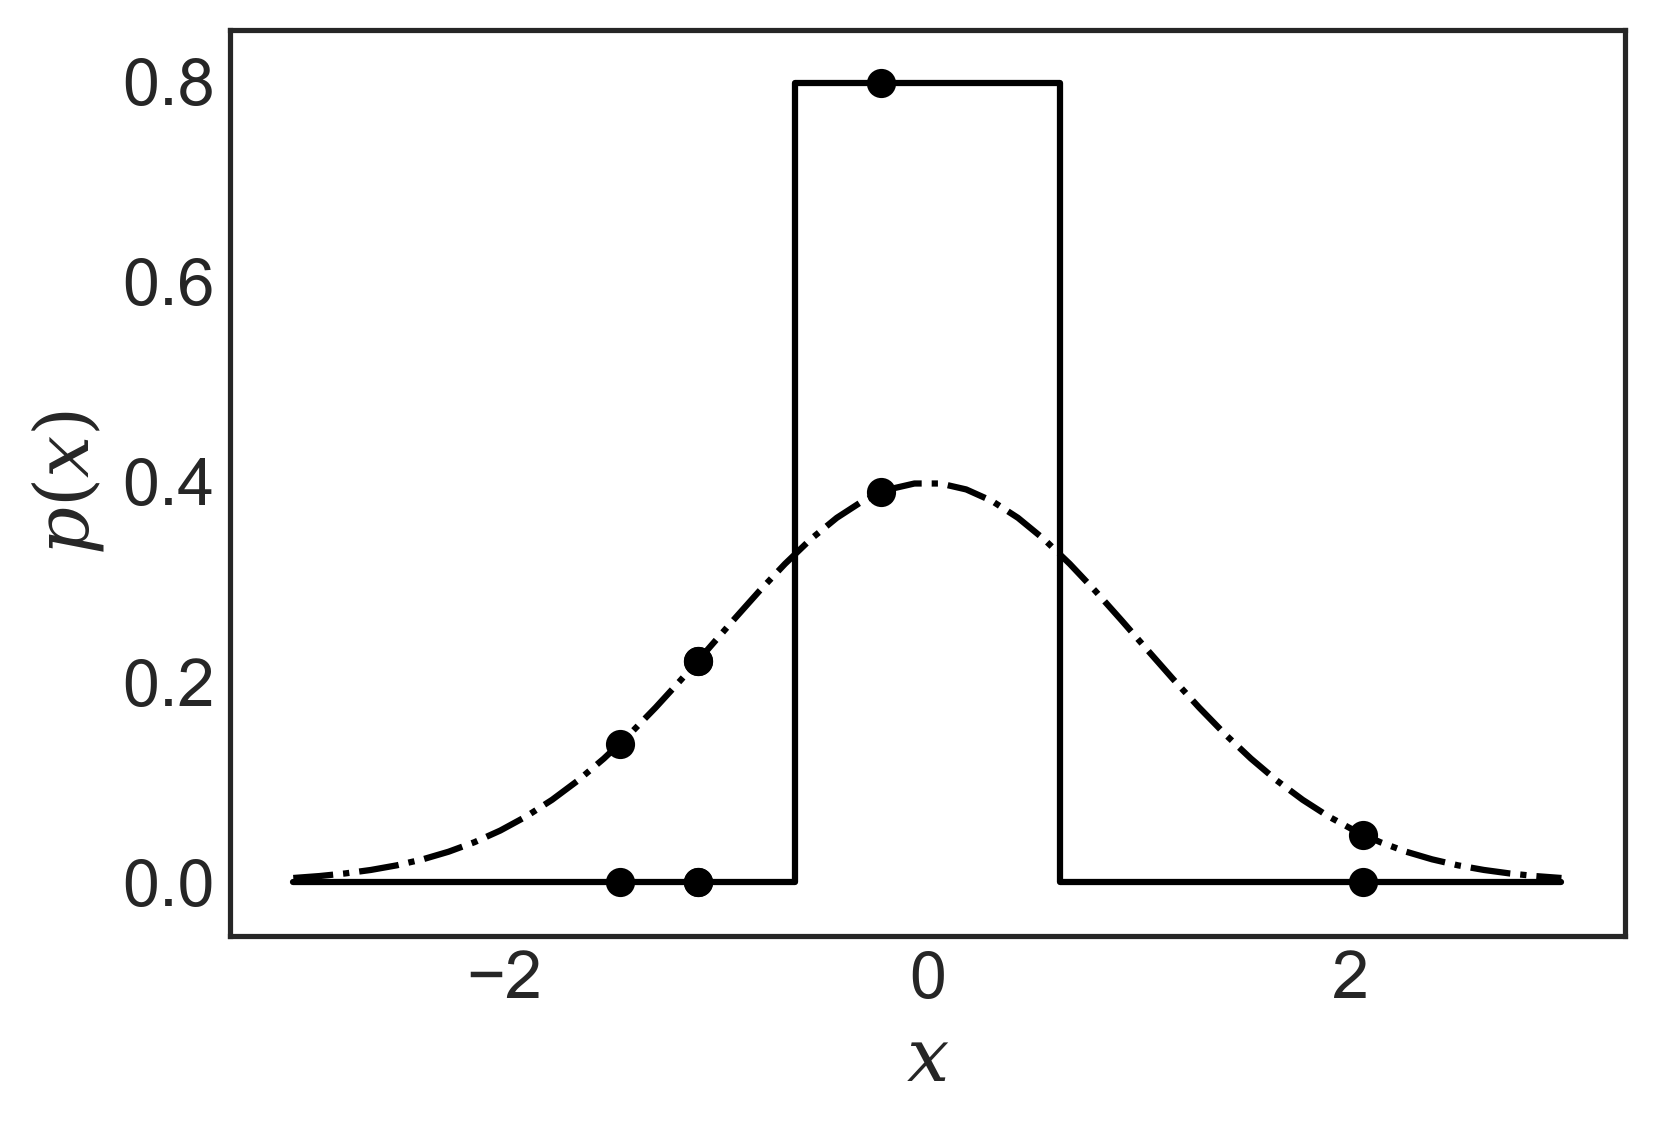
\includegraphics[height=3cm]{Gaussian_vs_box.png}%
\quad
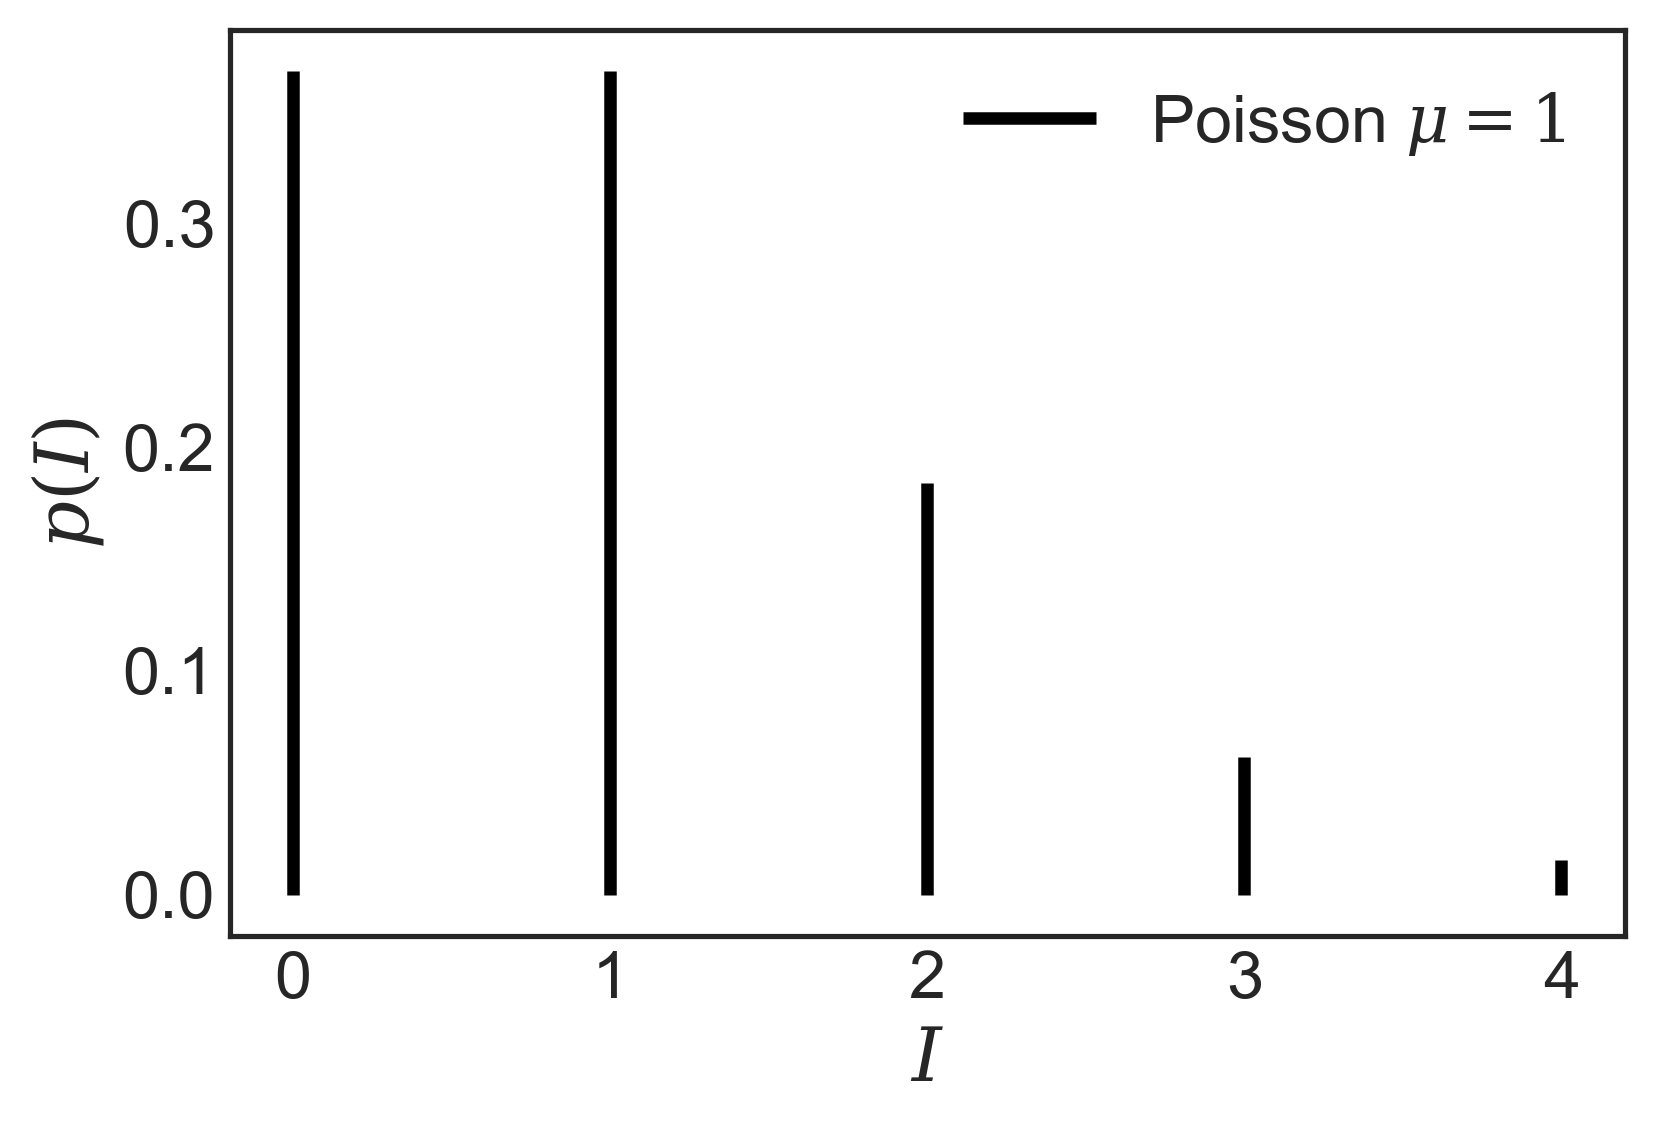
\includegraphics[height=3cm]{Poisson.png}%
}
\caption{The properties of a Poisson distribution can be employed to measure the concentration of dilute solutions of fluorescent molecules.}\label{fig:poissonconc}
\end{center}
\end{figure}

In single molecule techniques one often employs a Gaussian illumination profile to measure fluorescence intensities from a dilute solution of molecules.  Typically such measurements are performed by single photon detection and result in a sequence of single photon arrival times.  Several techniques have emerged from this approach: (1) Fluorescence correlation spectroscopy measures the concentration and diffusion coefficient of fluorescent molecules by analyzing the intensity autocorrelation function; (2) Photon Counting Histogram (PCH) is analyzing the distribution function of time-binned photon counts to measure the concentration and brightness of a dilute solution of fluorescent molecules.  In this article we develop a general framework for calculating the intensity distribution of a dilute solution of Point emitters under Gaussian Detection.  As compared to the Photon Counting Histogram method, we do not assume that the intensities are averaged over a time window but are taken as instantaneous snapshots of individual spacial emmiter distributions.  We will show that the resulting Intensity distributions dramatically change character at low emitter concentrations when considering different dimensionalities of the Gaussian Detection.  In particular the one- and two-dimensional solutions are strongly structured, exhibiting discontinuities in their derivative at integer multiples of the brightness.  This makes these distributions strong candidates to distinguish and measure concentrations of mixtures of emitters of different brightnesses.  Finally, we will discuss a maximum likelihood method to determine concentration and brightness from a sequence of single photon arrival times. 




\subsection{Intensity Probability Distribution}
In this section we will calculate the probability distribution of intensities from a single fluorescent particle confined in length $L$.  We write the probability of finding a particle at $x$ as:
\begin{equation}
	p(x) = \left\{
		\begin{array}{l@{\quad : \quad}l}
			\frac{1}{L} & -\frac{L}{2} \le x \le \frac{L}{2} \\
			0 & other \quad x
		\end{array}
	\right.
\end{equation}
The fluorescent intensity for a particle at position $x$ is proportional to the illumination profile given by:
\begin{equation}
	\Phi(x) = \Phi_{0}\exp{\left(-\frac{2x^{2}}{w^2}\right)}
\end{equation}
%In order to calculate $p(I)$ we need to evaluate the following integral
%\begin{equation}
%	p(\Phi)d\Phi = \int_{x:\Phi<\Phi(x)<\Phi+d\Phi} p(x)dx
%\end{equation}
%for all x for which the condition is fullfilled.  The integral can be evaluated by inverting $\Phi(x)$:
where $\Phi_{0}$ is specfic for each fluorescent species and includes all the contributions of quantum and detection efficiencies.  
We can calculate some of the properties of this intensity distribution function.  The expectation value of $\Phi^{n}$ is
\begin{equation}
	E[\Phi^{n}] = \sqrt{\frac{\pi}{2}}\frac{w}{L\sqrt{n}}\Phi_{0}^{n} \erf{\left(\sqrt{\frac{n}{2}}\frac{L}{w}\right)}
\end{equation}
all moments $E[\Phi^{n}]$ are inversely proportional to $L$.  When applied to a situation with fixed particle concentration $N/L$, $E[\Phi_{m}^{n}]$ is constant for large $L$ since $N$ goes up for larger $L$.\\
In order to find the intensity probability distribution at a certain concentration in an infinite volume (or length), we need to find the characteristic function of $p(\Phi)$.
\begin{equation}
	c(k) = \int_{\Phi(L/2)}^{\Phi_{0}}\exp(ik\Phi)p(\Phi)d\Phi
\end{equation}
by expanding the exponential function we see that
\begin{equation}
	\begin{aligned}
	c(k) &= \int_{\Phi(L/2)}^{\Phi_{0}}\sum_{n=0}^{\infty}\frac{(ik)^{n}\Phi^{n}}{n!}p(\Phi)\\
	&=1+\sum_{n=1}^{\infty}\frac{(ik)^{n}E[\Phi^{n}]}{n!}\\
	&=1+\sqrt{\frac{\pi}{2}}\frac{w}{L}\sum_{n=1}^{\infty}\frac{(ik)^{n}}{n!\sqrt{n}}\Phi_{0}^{n} \erf{\left(\sqrt{\frac{n}{2}}\frac{L}{w}\right)}
	\end{aligned}
\end{equation}
this characteristic function is for one particle in length $L$.  For more particles we need to convolute the probability distribution functions N times.  Alternatively we can take $c(k)$ to the power of N.  We can accomplish this by recognizing that the particle concentration is given by $c=N/L$ or $L=N/c$.  Inserting this into the previous equation we get:

\begin{equation}
	c(k) = 1+\sqrt{\frac{\pi}{2}}\frac{wc}{N}\sum_{n=1}^{\infty}\frac{(ik)^{n}}{n!\sqrt{n}}\Phi_{0}^{n} \erf{\left(\sqrt{\frac{n}{2}}\frac{N}{wc}\right)}
\end{equation}

In order to take $c(k)$ to the power of $N$ we will take advantage of two properties.  First,
\begin{equation}
\lim_{N\rightarrow \infty}\erf{\left(\sqrt{\frac{n}{2}}\frac{N}{wc}\right)} = 1
\end{equation}
and second,
\begin{equation}
\lim_{N\rightarrow \infty}\left(1+\frac{x}{N}\right)^{N} = \exp(x)
\end{equation}
combining both results in
\begin{equation}
	\lim_{N\rightarrow \infty}c(k) = C(k) = \exp\left(\sqrt{\frac{\pi}{2}}wc\sum_{n=1}^{\infty}\frac{(ik)^{n}}{n!\sqrt{n}}\Phi_{0}^{n} \right)
\end{equation}

Now we explore how the intensity probability distribution changes when considering higher dimensions.  For example, in a realistic experiment a confocal laser spot is often described as a three dimensional Gaussian intensity distribution:
\begin{equation}
	\Phi(x,y,z) = \Phi_{0}\exp{\left(-\frac{2(x^{2}+y^{2})}{w_{xy}^2}\right)}\exp{\left(-\frac{2z^{2}}{w_{z}^2}\right)}
\end{equation}
assuming that we calculate the expectation value of $\Phi^n$ in a box of $L^3$ for one fluorescent particle then we get
\begin{equation}
	E[\Phi^{n}] = \left(\frac{\pi}{2}\right)^{\frac{3}{2}}\frac{w_{xy}^{2}w_{z}}{L^{3}n^{\frac{3}{2}}}\Phi_{0}^{n} \erf{\left(\sqrt{\frac{n}{2}}\frac{L}{w_{xy}}\right)}^{2}\erf{\left(\sqrt{\frac{n}{2}}\frac{L}{w_{z}}\right)}
\end{equation}
which allows us to express the characteristic function as (using $c=N/L^{3}$)
\begin{equation}
	c(k) = 1+\left(\frac{\pi}{2}\right)^{\frac{3}{2}}\frac{cw_{xy}^{2}w_{z}}{N}\sum_{n=1}^{\infty}\frac{(ik)^{n}}{n!n^{\frac{3}{2}}}\Phi_{0}^{n} \erf{\left(\sqrt{\frac{n}{2}}\frac{1}{w_{xy}}\left(\frac{N}{c}\right)^{\frac{1}{3}}\right)}^{2}\erf{\left(\sqrt{\frac{n}{2}}\frac{1}{w_{z}}\left(\frac{N}{c}\right)^{\frac{1}{3}}\right)}
\end{equation}
As before we are taking the limit to to $N\rightarrow \infty$
\begin{equation}
	\lim_{N\rightarrow \infty}c(k) = C(k) = \exp\left(\left(\frac{\pi}{2}\right)^{\frac{3}{2}}cw_{xy}^{2}w_{z}\sum_{n=1}^{\infty}\frac{(ik)^{n}}{n!n^{\frac{3}{2}}}\Phi_{0}^{n}\right)
\end{equation}
similarily for 2d we get
\begin{equation}
	\lim_{N\rightarrow \infty}c(k) = C(k) = \exp\left(\frac{\pi}{2}cw_{xy}^{2}\sum_{n=1}^{\infty}\frac{(ik)^{n}}{n!n}\Phi_{0}^{n}\right)
\end{equation}
this form can be expressed as a function of special functions $Si$ and $Ci$ as follows
\begin{equation}
	\begin{aligned}
		Si(k)&=\int_{0}^{k}\frac{\sin t}{t}dt = \sum_{n=0}^{\infty}\frac{(-1)^{n}k^{2n+1}}{(2n+1)!(2n+1)}\\
		Ci(k)&=\gamma+\ln k +\int_{0}^{k}\frac{\cos t - 1}{t}dt=\gamma + \ln k + \sum_{n=1}^{\infty}\frac{(-1)^{n}k^{2n}}{(2n)!(2n)}
	\end{aligned}
\end{equation}
resulting in
\begin{equation}
	\begin{aligned}
	C(k) &= \exp\left(\frac{\pi}{2}cw_{xy}^{2}\left(Ci(k\Phi_{0})-\gamma-\ln k\Phi_{0}+iSi(k\Phi_{0})\right)\right)\\
	&=(k\Phi_{0})^{-\frac{\pi}{2}cw_{xy}^{2}}\exp\left(-\frac{\pi}{2}cw_{xy}^{2}\gamma\right)\exp\left(\frac{\pi}{2}cw_{xy}^{2}\left(Ci(k\Phi_{0})+iSi(k\Phi_{0})\right)\right)
	\end{aligned}
\end{equation}
for large $k$, $C(k)$ decays like
\begin{equation}
	\lim_{k\rightarrow \infty} C(k) = i(k\Phi_{0})^{-\frac{\pi}{2}cw_{xy}^{2}}\sin \left(\frac{\pi}{2}cw_{xy}^{2}\right)
\end{equation}
since the limiting values for $k\rightarrow \infty$ for $Ci(k\Phi_{0})$ is zero and for $Si(k\Phi_{0})$ is $\pi/2$
%\begin{equation}
%	C(k) = \exp\left(\frac{\pi}{2}cw_{xy}^{2}w_{z}\int_{0}^{1}\frac{\exp(ik\Phi_{0}y)-1}{y}dy \right)
%\end{equation}

\subsection{Integral representations of the exponent of $C(k)$}
Here we can take advantage of the integral representation of the gamma function
\begin{equation}
	\int_{0}^{\infty}t^{b}\exp(-nt)dt = \frac{\Gamma (b+1)}{n^{b+1}}
\end{equation}
For the 1-dimensional case, we are going to use
\begin{equation}
	\frac{1}{\sqrt{n}}=\frac{1}{\sqrt{\pi}}\int_{0}^{\infty}dt\frac{\exp(-tn)}{\sqrt{t}}
\end{equation}
\begin{equation}
	\begin{aligned}
	C(k) &= \exp\left(\frac{1}{\sqrt{2}}wc\int_{0}^{\infty}dt\frac{1}{\sqrt{t}}\sum_{n=1}^{\infty}\frac{(ik)^{n}}{n!}\Phi_{0}^{n}\exp(-tn) \right)\\
	&= \exp\left(\frac{1}{\sqrt{2}}wc\int_{0}^{\infty}dt\frac{1}{\sqrt{t}}(\exp(ik\Phi_{0}\exp(-t))-1) \right)\\
	&= \exp\left(\frac{1}{\sqrt{2}}wc\int_{0}^{\infty}dt\frac{\cos(k\Phi_{0}\exp(-t))-1+i\sin(k\Phi_{0}\exp(-t))}{\sqrt{t}} \right)
	\end{aligned}
\end{equation}
using a variable transform $y=\exp(-t)$ we find
\begin{equation}
	C(k) = \exp\left(\frac{1}{\sqrt{2}}wc\int_{0}^{1}dy\frac{\exp(ik\Phi_{0}y)-1}{y\sqrt{-\ln y}}\right)
\end{equation}
Similarly, in the 2-dimensional case, we find that
\begin{equation}
	\begin{aligned}
	C(k) &= \exp\left(\frac{\pi}{2}cw_{xy}^{2}\sum_{n=1}^{\infty}\frac{(ik)^{n}}{n!n}\Phi_{0}^{n}\right)\\
	&= \exp\left(\frac{\pi}{2}cw_{xy}^{2}\int_{0}^{\infty}dt(\exp(ik\Phi_{0}\exp(-t))-1) \right)\\
	&= \exp\left(\frac{\pi}{2}cw_{xy}^{2}\int_{0}^{\infty}dt\cos(k\Phi_{0}\exp(-t))-1+i\sin(k\Phi_{0}\exp(-t)) \right)
	\end{aligned}
\end{equation}
after a variable transform $y=\exp(-t)$ we find
\begin{equation}
	\begin{aligned}
	C(k) &= \exp\left(\frac{\pi}{2}cw_{xy}^{2}\int_{0}^{1}dy\frac{\exp(ik\Phi_{0}y)-1}{y}\right)\\
	&= \exp\left(\frac{\pi}{2}cw_{xy}^{2}\int_{0}^{k\Phi_{0}}dx\frac{\exp(ix)-1}{x}\right)\\
	&= \exp\left(-\frac{\pi}{2}cw_{xy}^{2}Ein(k\Phi_{0})\right)
	\end{aligned}
\end{equation}
where $Ein(x)$ is related to the Exponential Integral $E_{1}(x) = -\gamma -\ln x +Ein(x)$, which clarifies the connection to the Trigonometic integrals in the previous section.

Similarly, in the 3-dimensional case, we can get
\begin{equation}
	\begin{aligned}
	C(k) &= \exp\left(\frac{\pi}{\sqrt{2}}cw_{xy}^{2}w_{z}\int_{0}^{\infty}dt\sqrt{t}\sum_{n=1}^{\infty}\frac{(ik)^{n}}{n!}\Phi_{0}^{n}\exp(-tn)\right)\\
	&= \exp\left(\frac{\pi}{\sqrt{2}}cw_{xy}^{2}w_{z}\int_{0}^{\infty}dt\sqrt{t}(\exp(ik\Phi_{0}\exp(-t))-1) \right)
	\end{aligned}
\end{equation}
and after a variable transform $y=\exp(-t)$ we find
\begin{equation}
	C(k) = \exp\left(\frac{\pi}{\sqrt{2}}cw_{xy}^{2}w_{z}\int_{0}^{1}\frac{\sqrt{-\ln{y}}}{y}(\exp(ik\Phi_{0}y)-1)dy \right)
\end{equation}

\begin{acknowledgments}
We wish to acknowledge funding by the NSF (DMR Award
1106044), the NIH (5R21DA03846702), and discussions with Alexei Borodin, Nikita Nikrasov, Eugene and Joachim R\"adler.
\end{acknowledgments}

\end{document}
